\documentclass[a4paper,12pt]{report}
\usepackage[utf8]{inputenc}
\usepackage[T1]{fontenc}
\usepackage[french]{babel} 
\usepackage{pdfpages}
\usepackage{xcolor,graphicx}
\usepackage{enumitem}
\usepackage{hyperref}
\usepackage[top=1cm, bottom=2cm, left=1cm, right=1cm]{geometry}
\graphicspath{{image/}}
\usepackage{graphicx}
\bibliographystyle{unsrt}
\usepackage{array}
\linespread{1.5}




\begin{document}

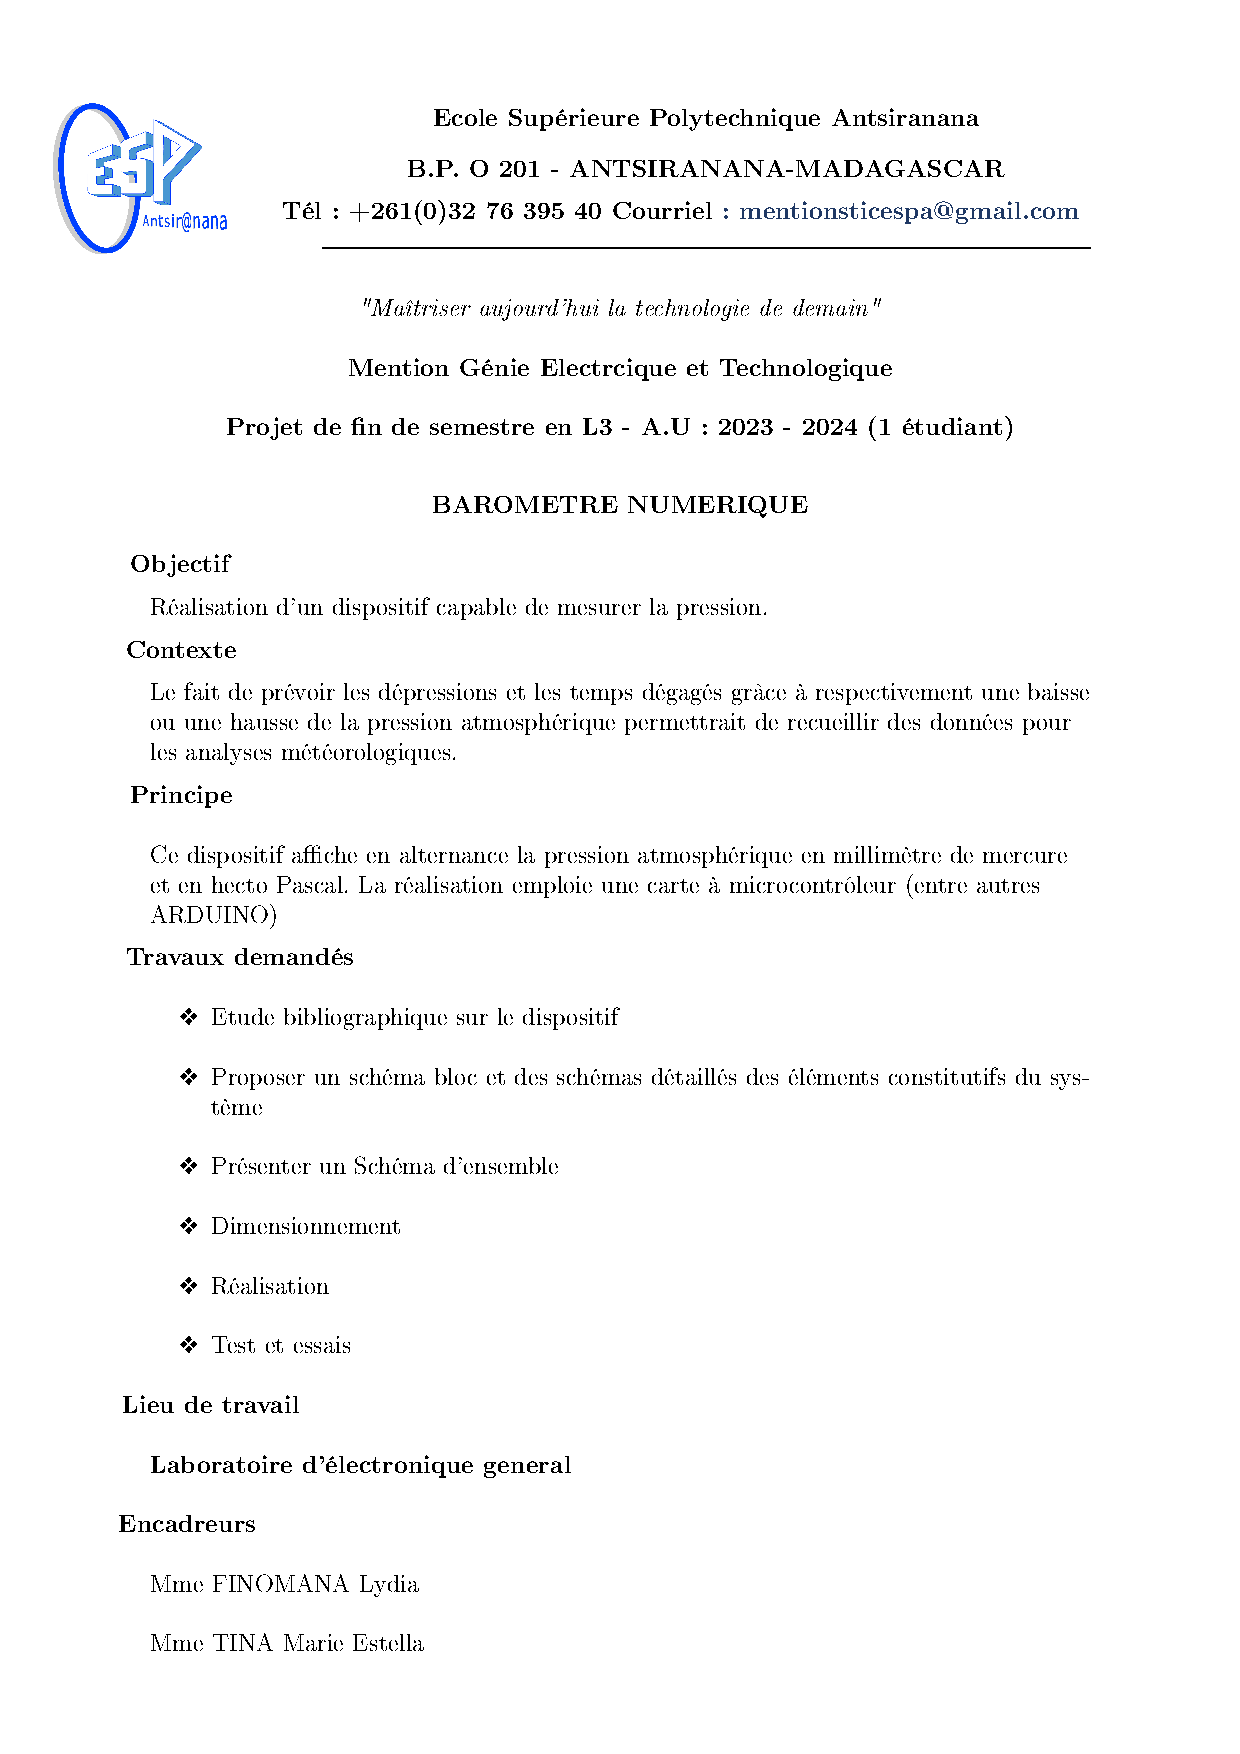
\includepdf[pages={1}]{cahier de charge.pdf}

\pagebreak

\pagestyle{empty}

Dans ce rapport \cite{barometer} les auteurs ont pour objectif d'afficher la pression atmosphérique en Pa sur un écran LCD à l'aide d'un capteur,d'un convertisseur analogique-numérique et d'un décodeur LCD. Le capteur utilisé est le MPX2200AP.\\

Les articles suivants utilisent tous des cartes à microcôntroleurs et la famille de capteur BMP de la marque BOSCH.\\

\url{https://pic-in-pascal.blogspot.com/2017/07/barometric-pressure-sensor.html}\\[1cm]
\url{https://circuitdigest.com/microcontroller-projects/pressure-sensor-bmp180-with-arduino}\\[1cm]
\url{srituhobby.com/bmp180-sensor-with-arduino}\\[1cm]


\bibliographystyle{plain}
\bibliography{biblio} 











\end{document}